% This file was created by matlab2tikz.
%
%The latest updates can be retrieved from
%  http://www.mathworks.com/matlabcentral/fileexchange/22022-matlab2tikz-matlab2tikz
%where you can also make suggestions and rate matlab2tikz.
%
\definecolor{mycolor1}{rgb}{0.00000,0.44700,0.74100}%
\definecolor{mycolor2}{rgb}{0.85000,0.32500,0.09800}%
\definecolor{mycolor3}{rgb}{0.92900,0.69400,0.12500}%
%
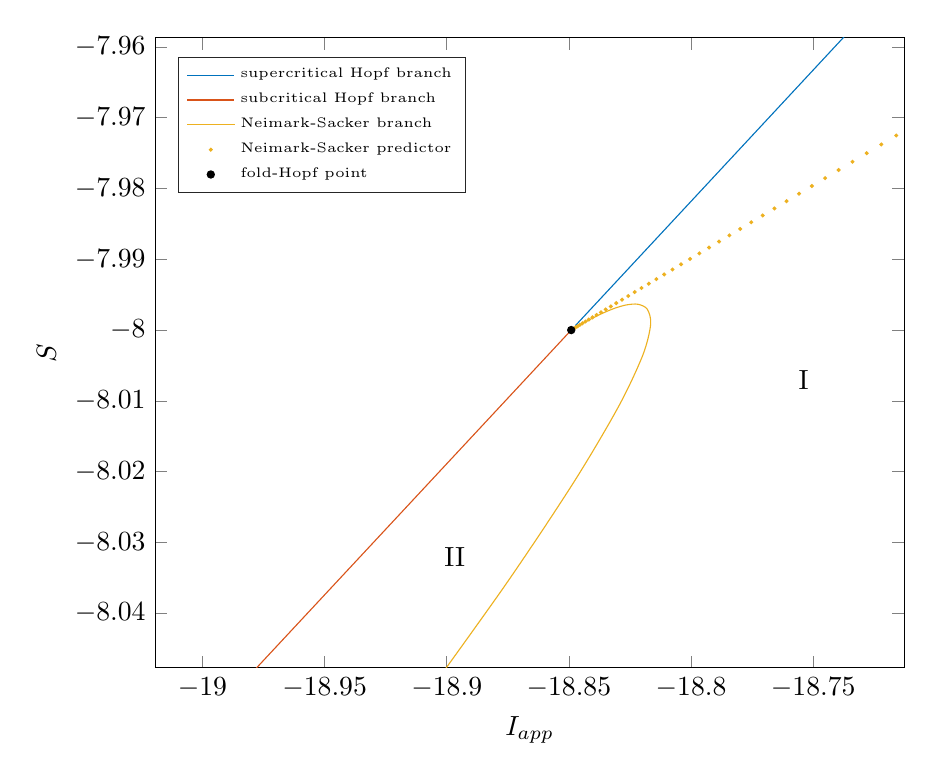
\begin{tikzpicture}[%
mark size=0.5
]

\begin{axis}[%
width=9.509cm,
height=8cm,
at={(0cm,0cm)},
scale only axis,
xmin=-19.0193,
xmax=-18.7128,
xlabel={$I_{app}$},
ymin=-8.0477,
ymax=-7.9587,
ylabel={$S$},
axis background/.style={fill=white},
legend style={at={(0.03,0.97)},anchor=north west,legend cell align=left,align=left,draw=white!15!black,font=\tiny}
]
\addplot [color=mycolor1,solid]
  table[row sep=crcr]{%
-18.8473611635171	-7.99937663262835\\
-18.8453435786192	-7.99862857396533\\
-18.8429224616458	-7.99773087791389\\
-18.8400170995462	-7.99665360570904\\
-18.8365306337442	-7.99536082586726\\
-18.8323468297544	-7.99380941345869\\
-18.8273262001602	-7.99194760827308\\
-18.8213013513833	-7.98971328323613\\
-18.8140713986497	-7.98703186451844\\
-18.8053952622902	-7.98381383280051\\
-18.7953950012695	-7.98010432648132\\
-18.7853947220817	-7.97639443995615\\
-18.7753944432488	-7.97268418006628\\
-18.7653941647705	-7.96897354678254\\
-18.7553938866461	-7.96526254007558\\
-18.745393608875	-7.96155115991597\\
-18.7353933314566	-7.95783940627421\\
};
\addlegendentry{supercritical Hopf branch};

\addplot [color=mycolor2,solid]
  table[row sep=crcr]{%
-18.9840827111782	-8.0500334008489\\
-18.974082996765	-8.04633076532673\\
-18.9640832819851	-8.0426277567487\\
-18.9540835668391	-8.0389243750874\\
-18.9440838513277	-8.03522062031534\\
-18.9340841354515	-8.03151649240495\\
-18.9240844192113	-8.0278119913286\\
-18.9140847026077	-8.02410711705855\\
-18.9040849856415	-8.0204018695671\\
-18.8940852495942	-8.01669624188913\\
-18.8854110644888	-8.01348152477592\\
-18.8781824145905	-8.01080231919396\\
-18.8721584270594	-8.00856945716304\\
-18.8671383593024	-8.00670860637588\\
-18.862954915269	-8.00515780542915\\
-18.8594686742633	-8.00386540745132\\
-18.8565634472944	-8.00278836479449\\
-18.8541424066802	-8.00189079845536\\
-18.8521248602416	-8.00114280512363\\
-18.8504435627995	-8.00051946249868\\
-18.8490424755272	-8\\
};
\addlegendentry{subcritical Hopf branch};

\addplot [color=mycolor3,solid,smooth]
  table[row sep=crcr]{%
-18.8487603703132	-7.99994171113551\\
-18.8487546999984	-7.99994053952934\\
-18.8487486358889	-7.99993942259773\\
-18.8487400591522	-7.99993761532994\\
-18.8487299196219	-7.99993552840346\\
-18.8487175342639	-7.99993297961539\\
-18.8487024267362	-7.99992988250462\\
-18.8486837646326	-7.99992604354951\\
-18.8486607218207	-7.99992130474171\\
-18.8486321853961	-7.99991544589103\\
-18.8485965467623	-7.99990812227151\\
-18.8485518582983	-7.99989894379846\\
-18.8484954604888	-7.99988736577651\\
-18.848423847075	-7.99987267953981\\
-18.8483322519174	-7.99985391586253\\
-18.8482142959217	-7.99982979353187\\
-18.8480611583993	-7.9997985233994\\
-18.8478609934438	-7.99975774822529\\
-18.8475976921119	-7.99970430244309\\
-18.8472488778343	-7.99963377384223\\
-18.8467845896362	-7.9995404397951\\
-18.8461644779168	-7.99941681136286\\
-18.8453340168076	-7.99925302365018\\
-18.8442229041109	-7.99903730862433\\
-18.8427424339044	-7.99875641490087\\
-18.840785672428	-7.99839743781698\\
-18.8382378312266	-7.99795379300436\\
-18.8349985625584	-7.99743581706918\\
-18.8310348662484	-7.99689241530226\\
-18.8264768250186	-7.99644688610363\\
-18.8217777396217	-7.99635156483045\\
-18.8179185632359	-7.99704796034447\\
-18.8165282228965	-7.99918175499532\\
-18.8197105242569	-8.00351120872758\\
-18.8295793145536	-8.01074437586913\\
-18.8479493857823	-8.0214696487906\\
-18.8764327299462	-8.03622584064449\\
-18.9167262497052	-8.05561130615932\\
};
\addlegendentry{Neimark-Sacker branch};

\addplot [color=mycolor3,only marks,mark=*,mark options={solid}]
  table[row sep=crcr]{%
-18.8490424755272	-8\\
-18.8489705172541	-7.99998513190886\\
-18.8487546424347	-7.99994052763546\\
-18.8483948510691	-7.99986618717978\\
-18.8478911431572	-7.99976211054183\\
-18.8472435186991	-7.99962829772161\\
-18.8464519776947	-7.99946474871912\\
-18.845516520144	-7.99927146353435\\
-18.8444371460472	-7.99904844216732\\
-18.843213855404	-7.99879568461801\\
-18.8418466482146	-7.99851319088643\\
-18.840335524479	-7.99820096097258\\
-18.8386804841971	-7.99785899487646\\
-18.836881527369	-7.99748729259807\\
-18.8349386539946	-7.99708585413741\\
-18.8328518640739	-7.99665467949447\\
-18.830621157607	-7.99619376866927\\
-18.8282465345939	-7.99570312166179\\
-18.8257279950345	-7.99518273847204\\
-18.8230655389288	-7.99463261910002\\
-18.8202591662769	-7.99405276354573\\
-18.8173088770788	-7.99344317180917\\
-18.8142146713344	-7.99280384389033\\
-18.8109765490437	-7.99213477978923\\
-18.8075945102068	-7.99143597950585\\
-18.8040685548237	-7.9907074430402\\
-18.8003986828943	-7.98994917039228\\
-18.7965848944186	-7.98916116156209\\
-18.7926271893967	-7.98834341654963\\
-18.7885255678286	-7.9874959353549\\
-18.7842800297141	-7.98661871797789\\
-18.7798905750535	-7.98571176441861\\
-18.7753572038466	-7.98477507467707\\
-18.7706799160934	-7.98380864875325\\
-18.765858711794	-7.98281248664716\\
-18.7608935909483	-7.9817865883588\\
-18.7557845535564	-7.98073095388816\\
-18.7505315996182	-7.97964558323526\\
-18.7451347291338	-7.97853047640008\\
-18.7395939421031	-7.97738563338264\\
-18.7339092385262	-7.97621105418292\\
-18.728080618403	-7.97500673880093\\
-18.7221080817336	-7.97377268723667\\
-18.7159916285179	-7.97250889949013\\
-18.709731258756	-7.97121537556133\\
};
\addlegendentry{Neimark-Sacker predictor};

\addplot [color=black,mark size=1.3pt,only marks,mark=*,mark options={solid}]
  table[row sep=crcr]{%
-18.8490424755272	-8\\
};
\addlegendentry{fold-Hopf point};

\node[right, align=left, text=black]
at (axis cs:-18.76,-8.007) {I};
\node[right, align=left, text=black]
at (axis cs:-18.905,-8.032) {II};
\end{axis}
\end{tikzpicture}%